\documentclass{article}
\usepackage[margin=1in]{geometry}
\usepackage{graphicx}
\usepackage[dvipsnames,table]{xcolor}
\usepackage[utf8]{inputenc}
\usepackage{siunitx}
\usepackage[american,siunitx]{circuitikz}
\usepackage{amsmath}
\usepackage{svg}
\usepackage{booktabs}
\usepackage{float}
\usepackage{xparse, xfp}
\usepackage{multirow}
\usepackage{tikz}
\usepackage{karnaugh-map}
\usepackage{pdfpages}
\usepackage{hyperref}
\usepackage{adjustbox}
\usepackage{listings}
\usepackage[shortlabels]{enumitem}

\definecolor{codegreen}{rgb}{0,0.6,0}
\definecolor{codegray}{rgb}{0.5,0.5,0.5}
\definecolor{codepurple}{rgb}{0.58,0,0.82}
\definecolor{backcolour}{rgb}{0.95,0.95,0.92}

\lstdefinestyle{mystyle}{
    backgroundcolor=\color{backcolour},   
    commentstyle=\color{codegreen},
    keywordstyle=\color{magenta},
    numberstyle=\tiny\color{codegray},
    stringstyle=\color{codepurple},
    basicstyle=\ttfamily\footnotesize,
    breakatwhitespace=false,         
    breaklines=true,                 
    captionpos=b,                    
    keepspaces=true,                 
    numbers=left,                    
    numbersep=5pt,                  
    showspaces=false,                
    showstringspaces=false,
    showtabs=false,                  
    tabsize=2
}
\lstset{style=mystyle}


\hypersetup{
    colorlinks=true,
    linkcolor=blue,
    filecolor=magenta,      
    urlcolor=cyan,
}
\usetikzlibrary{calc}
%\usepackage[landscape]{geometry}
\renewcommand{\thesubsection}{\thesection.\alph{subsection}}
\newcommand{\equal}{=}
\newcommand{\greyrule}{\arrayrulecolor{black!30}\midrule\arrayrulecolor{black}}
\makeatletter
\newcommand\currcoor{\the\tikz@lastxsaved,\the\tikz@lastysaved}
\makeatother
\newcolumntype{:}{@{\hskip\tabcolsep\color{black!30}\vrule\hskip\tabcolsep}}

\ExplSyntaxOn
\NewExpandableDocumentCommand \groupify { O{\,\allowbreak} m m }
  { \jakob_groupify:nnn {#1} {#2} {#3} }
\cs_new:Npn \jakob_groupify:nnn #1 #2 #3
  { \__jakob_groupify_loop:nnw { 1 } {#2} #3 \q_recursion_tail {#1} \q_recursion_stop }
\cs_new:Npn \__jakob_groupify_loop:nnw #1 #2 #3
  {
    \quark_if_recursion_tail_stop:n {#3}
    \exp_not:n {#3}
    \int_compare:nNnTF {#1} = {#2}
      { \__jakob_groupify_sep:n }
      { \exp_args:Nf \__jakob_groupify_loop:nnw { \int_eval:n { #1+1 } } }
          {#2}
  }
\cs_new:Npn \__jakob_groupify_sep:n #1 #2 \q_recursion_tail #3
  {
    \tl_if_empty:nF {#2} { \exp_not:n {#3} }
    \__jakob_groupify_loop:nnw { 1 } {#1}
    #2 \q_recursion_tail {#3}
  }
\ExplSyntaxOff

\title{ECE 4310\\Operating Systems for Embedded Application\\\,\\Quiz 2}
\author{Choi Tim Antony Yung}
%\date{February 11, 2021}
\begin{document}
\maketitle

\thispagestyle{empty}
\setcounter{page}{0}

\newpage




\section{(25 pts) Consider the following processes arriving at the ready queue and dispatched to a single core CPU using preemptive shortest job first scheduling:}

\begin{table}[H]
  \centering
  \begin{tabular}{r|ccc}
    \toprule
    \multirow{2}{*}{PID} & Arrival & Burst & Priority\\
                         & Time    & (ms)  &\\
    \midrule
    10                   & 0       & 18    &10\\
    11                   & 4       & 4    &2\\
    12                   & 9       & 6    &7\\
    13                   & 16      & 9    &3\\
    14                   & 23      & 2    &8\\
    \bottomrule
  \end{tabular}
\end{table}

Answer the following:\\
\begin{enumerate}[(a)]
  \item Draw a Gantt chart showing the arrival time and run times for each process.
  \item Calculate the wait time for each process and average waiting time.
  \item Calculate the turnaround time for each process.
\end{enumerate}

\begin{adjustbox}{max width=\textwidth}
  \begin{tikzpicture}
    % draw horizontal line   
    \draw (0,0) -- (39,0);

    % draw vertical lines
    \foreach \x in {0,4,8,9,15,16,25,37,39}
    \draw (\x cm,10pt) -- (\x cm,-10pt);

    % draw nodes
    \draw ( 0,0) node[below=10pt] {\Large$ 0 $} node[above=10pt] {\huge$   $};
    \draw ( 4,0) node[below=10pt] {\Large$ 4 $} node[above=10pt] {\huge$   $};
    \draw ( 8,0) node[below=10pt] {\Large$ 8 $} node[above=10pt] {\huge$   $};
    \draw ( 9,0) node[below=10pt] {\Large$ 9 $} node[above=10pt] {\huge$   $};
    \draw (15,0) node[below=10pt] {\Large$ 15 $} node[above=10pt] {\huge$   $};
    \draw (16,0) node[below=10pt] {\Large$ 16 $} node[above=10pt] {\huge$   $};
    \draw (25,0) node[below=10pt] {\Large$ 25 $} node[above=10pt] {\huge$   $};
    \draw (37,0) node[below=10pt] {\Large$ 37 $} node[above=10pt] {\huge$   $};
    \draw (39,0) node[below=10pt] {\Large$ 39 $} node[above=10pt] {\huge$   $};


    \draw (2,0)  node[below=10pt] {\Large$  $} node[above=10pt] {\Large 10};
    \draw (6,0)    node[below=10pt] {\Large$  $} node[above=10pt] {\Large 11};
    \draw (8.5,0)  node[below=10pt] {\Large$  $} node[above=10pt] {\Large 10};
    \draw (12,0)  node[below=10pt] {\Large$  $} node[above=10pt] {\Large 12};
    \draw (15.5,0) node[below=10pt] {\Large$  $} node[above=10pt] {\Large 10};
    \draw (20.5,0) node[below=10pt] {\Large$  $} node[above=10pt] {\Large 13};
    \draw (31,0) node[below=10pt] {\Large$  $} node[above=10pt] {\Large 10};
    \draw (38,0) node[below=10pt] {\Large$  $} node[above=10pt] {\Large 14};

  \end{tikzpicture}
\end{adjustbox}
\begin{table}[H]
  \centering
  \begin{tabular}{r|rr}
    \toprule
    \multirow{2}{*}{PID} & Wait      & Turnaround \\
            & Time      & Time       \\
    \midrule
    10      & $(25-16)+(15-9)+(8-4)+(0-0)=19$ & $37-0 =37$ \\
    11      & $ 4-4 =0$              & $ 8-4 =4 $ \\
    12      & $ 9-9 =0$              & $15-9 =6 $ \\
    13      & $16-16=0$              & $25-16=9 $ \\
    14      & $37-23=14$    & $39-23=16 $ \\
    \bottomrule
  \end{tabular}
\end{table}
$\text{Average wait time} = \frac{1}{5}(19+0+0+0+16)=7$

\section{(25 pts) Many round-robin schedulers use a fixed size quantum. Provide an argument in favor of and against a small quantum. Thoroughly explain your answer.}
An advantage of a smaller quantum is that process that have a larger burst time sees a decrease in turnaround time as it get allocated time slices more frequently. 
The disadvantage of a small quantum is that there are more switching between processes as quantum get smaller and more context switching means more overhead. 
Also, smaller processes sees their wait time and turnaround time increase as they may otherwise finish in one time slice where the quantum size bigger.

\end{document}